\begin{figure*}
  \centering
  \begin{minipage}{0.30\linewidth}
    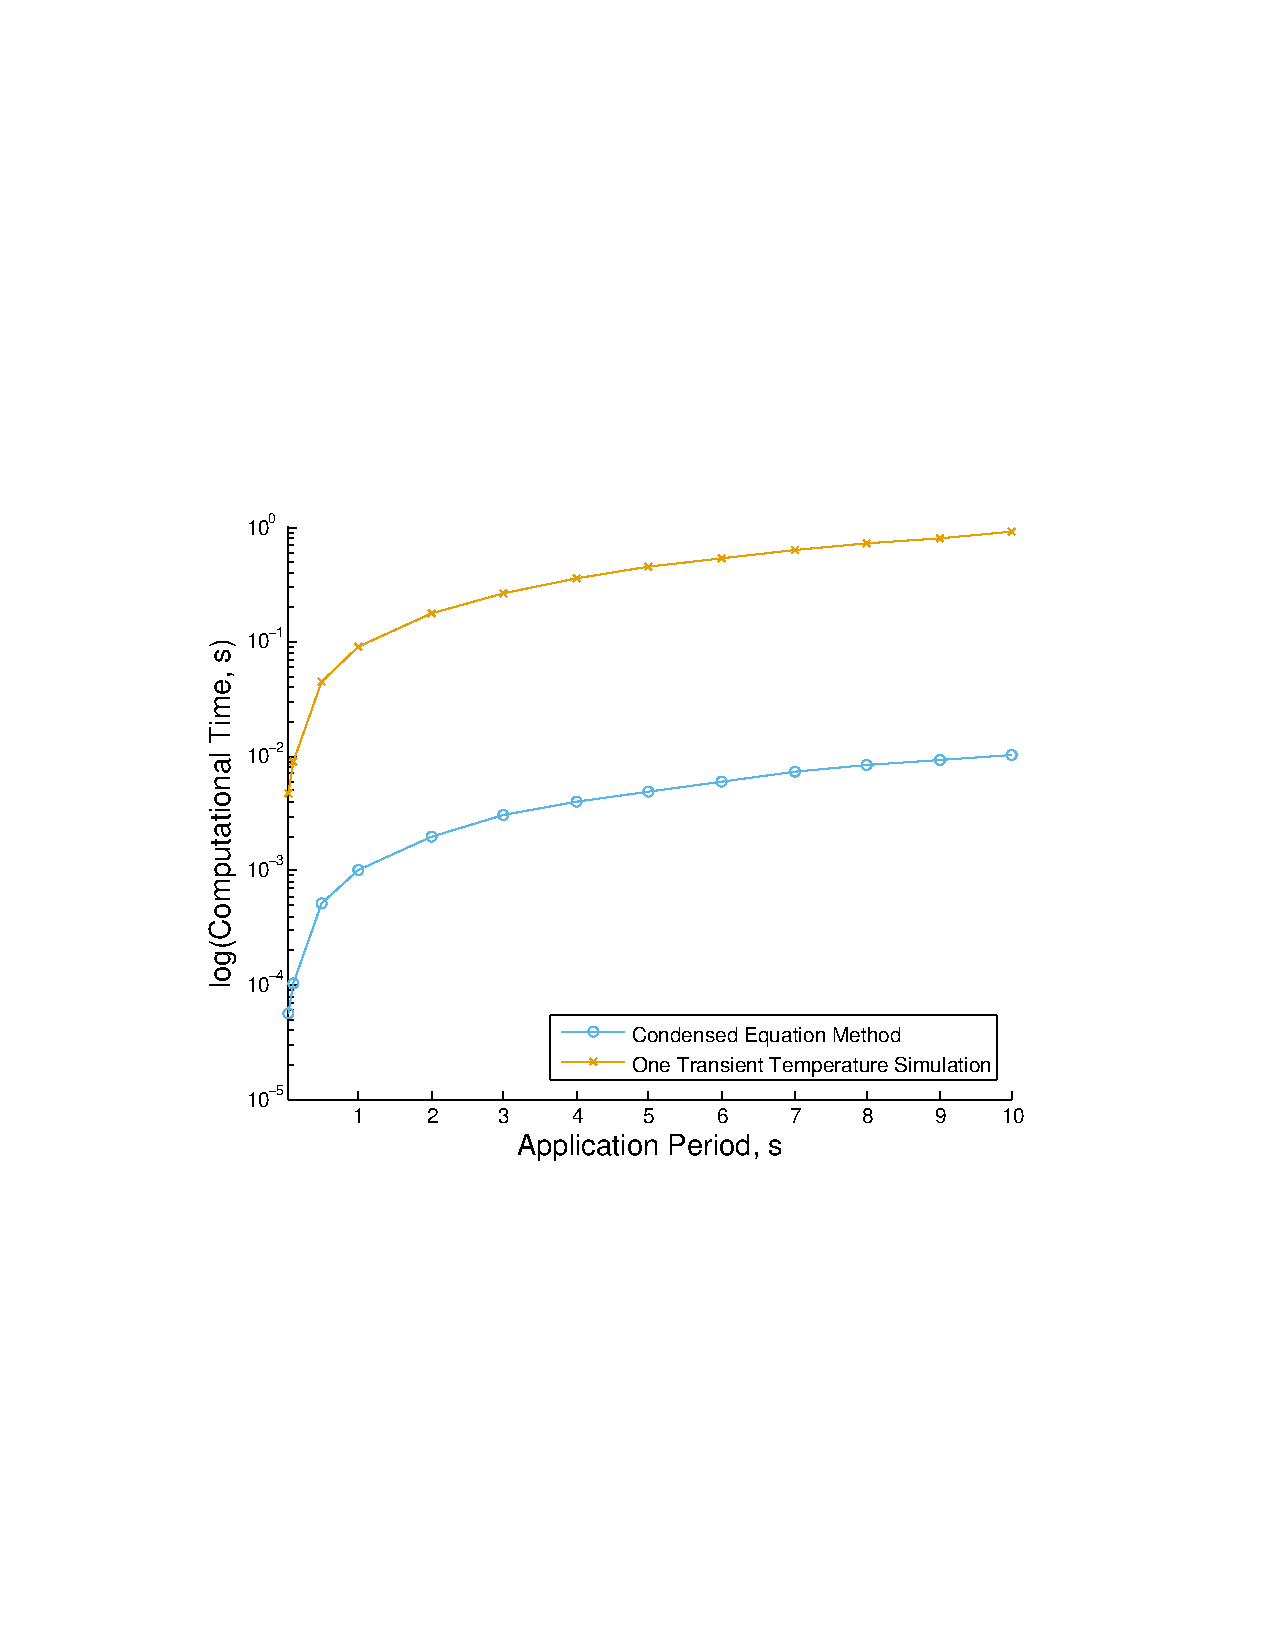
\includegraphics[clip=true, trim=15 0 15 0, width=\linewidth]{assets/scaling-time.pdf}
    \caption{Scalability with $\period$.}
    \label{fig:scaling-time}
  \end{minipage}
  \begin{minipage}{0.30\linewidth}
    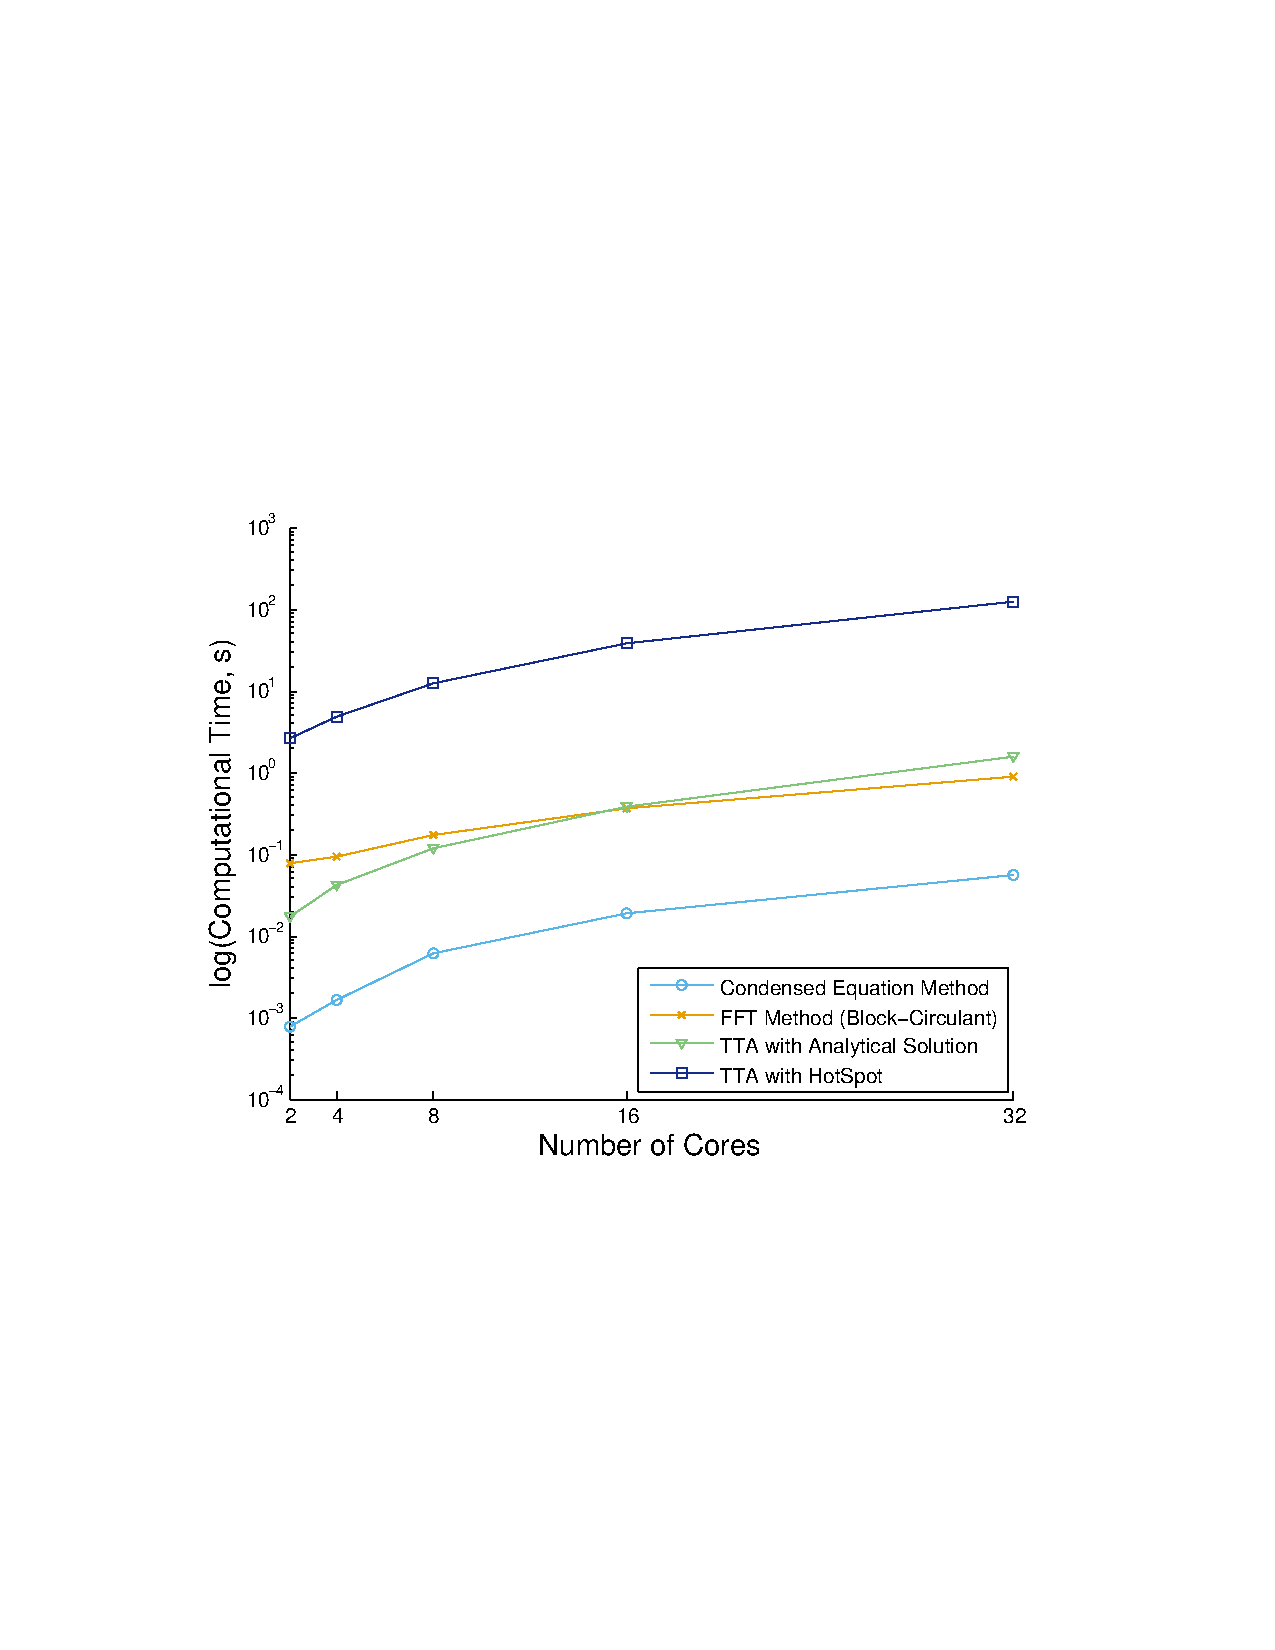
\includegraphics[clip=true, trim=15 0 15 0, width=\linewidth]{assets/scaling-cores.pdf}
    \caption{Scalability with $N_p$.}
    \label{fig:scaling-cores}
  \end{minipage}
  \begin{minipage}{0.35\linewidth}
    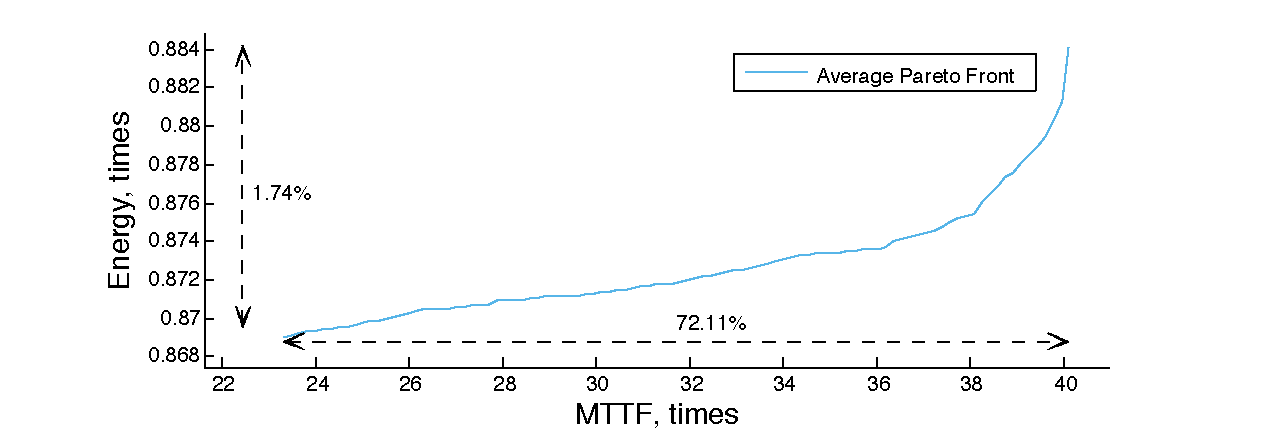
\includegraphics[clip=true, trim=50 0 50 0, width=\linewidth]{assets/average-pareto.pdf}
    \caption{Average Pareto front.}
    \label{fig:average-pareto}
  \end{minipage}
\end{figure*}

So far, we have assumed that power is independent of temperature. However, due to the leakage component, the power dissipation is a strong function of temperature that cannot be neglected (\secref{sec:power-model}). Two techniques can be applied to include in our proposed solution temperature dependent leakage modeling.

\subsection{Iterative Computation} \label{sec:iterative-leakage}
In this case, we have an iterative process, depicted in \figref{fig:leakage}, where the temperature and power profiles are calculated in turns. With each new temperature profile we update the power profile by computing the leakage power and adding it to the dynamic power: $\mathbb{P}_i = \mathbb{P}_{dyn} + \mathbb{P}_{leak}(\mathbb{T}_i)$. The process continues until the temperature converges, i.e., the difference between two successive temperature profiles is below a predefined bound. In our experiments we used $0.5^\circ C$ as the maximal acceptable difference and observed that the number of required iterations to converge is 4--7.

\subsection{Linear Approximation} \label{sec:linearized-leakage}
A linear approximation of the leakage power has the following matrix form: $\v{P}_{leak}(\v{T}) = \m{A} \: \v{T}(t) + \v{B}$ where $\m{A}$ is a $N_n \times N_n$ diagonal matrix of the proportionality and $\v{B}$ is a vector with $N_n$ elements of the intercept. Both characterize the leakage power for each of the $N_n$ thermal nodes in the system. It can be seen that the approximation keeps \equref{eq:fourier-model} untouched: $\m{C} \: \frac{d\v{T}(t)}{dt} + \bar{\m{G}} \: (\v{T}(t) - \v{T}_{amb}) = \bar{\v{P}}$ where $\bar{\m{G}} = \m{G} - \m{A}$ and $\bar{\v{P}} = \v{P}_{dyn} + \m{A} \: \v{T}_{amb} + \v{B}$. Therefore, all solutions proposed in this paper are perfectly valid with the linearized model. Moreover, in spite of its simplicity, the model provides a good estimation as shown in \cite{liu2007}.

In order to evaluate the linearization, we have constructed a number of hypothetical platforms with 2--32 cores (other parameters are given in \tabref{tab:parameters}) and compared temperature profiles obtained with the linearization and the exponential model (\secref{sec:power-model}), respectively. For the later, we use the iterative approach described above. For the linearization, the power curve fitting with the least squares regression \cite{press2007} has been employed, targeted at the range between 40 and $80^\circ C$. From the experiments we have observed that the NRMSE is bounded by 1--2\%, indicating a good accuracy of the linear approximation.
